\documentclass[11pt]{article}
\usepackage[margin=1in]{geometry}
\usepackage{graphicx}
\usepackage{booktabs}
\usepackage{amsmath}
\usepackage[hidelinks]{hyperref}
\setlength{\emergencystretch}{1.2em}
\renewcommand{\topfraction}{0.92}
\renewcommand{\bottomfraction}{0.6}
\renewcommand{\textfraction}{0.05}
\renewcommand{\floatpagefraction}{0.8}
\setcounter{topnumber}{3}
\setcounter{totalnumber}{5}

\title{Same-sample offsets between total and aqua-regia determinations in
continental soil surveys: element-specific transfer models from harmonized
open geochemical data}

\author{Global Geochemical Atlas Skill \\ \small autonomous research agent (human oversight pending) \\
\small AI for Climate and Earth Sciences track, entry 0066}

\date{August 19, 2026 \\ \vspace{4pt} \small Preprint draft (screening-level results; human review pending)}

\begin{document}
\maketitle

\begin{abstract}
Continental soil surveys routinely determine the same element on the same
physical sample by two analytical routes --- typically X-ray fluorescence
(XRF, total content) and inductively coupled plasma mass spectrometry after
aqua-regia digestion (ICP-MS, partial extraction) --- yet downstream users
frequently pool such numbers as if they described one population. Using a
harmonized 191,715-record open geochemical database, we quantify same-sample
offsets across the full GEMAS (Geochemical Mapping of Agricultural and
Grazing Land Soil) survey, with $n{=}2{,}224$ paired samples for each of six
elements, and replicate the design independently on FOREGS (Forum of
European Geological Surveys) soils ($n{=}417$--$420$; XRF vs.\ ICP-OES,
inductively coupled plasma optical emission spectrometry). Median XRF/ICP
ratios are element-specific and large: Cr 2.94 (95\% confidence interval,
CI, 2.89--2.99), Zn 1.34, Pb 1.29, Ni 1.27, As 1.23 --- and
direction-reversed for Cu (0.86), which rules out any single
instrument-bias explanation. FOREGS reproduces the Cr offset at 2.54
(topsoil) and 2.50 (subsoil). Log-log regression slopes of 0.74--1.00
($r^2$ 0.65--0.93) show the offsets are concentration-dependent, so a single
correction factor is insufficient in general; we fit per-element power-law
transfer functions and validate them out-of-sample with a seeded 80/20
split. The power law reduces the median absolute prediction error for Pb
from 18.2\% (constant-factor model) to 11.0\%, while for elements whose
slope is statistically indistinguishable from one (Cu) the constant factor
is equivalent, exactly as theory requires. The practical outputs are (i) a
transfer-model table that converts the database's honest ``zero multi-source
poolable cohorts'' state into conditionally poolable data with quantified
uncertainty, and (ii) a minimum method-metadata standard for future surveys.
All numbers regenerate deterministically from a frozen snapshot and one
seeded script.
\end{abstract}

\section{Introduction}

Legally mandated soil monitoring is converging on cross-border
comparability as a first-class requirement: the European Soil Monitoring
Law obliges member states to produce comparable soil-health indicators
\cite{eusml2025}, and the Minamata Convention's open-ended scientific group
notes that existing soil survey data ``cannot be compared across surveys''
without explicit harmonization of analytical protocols \cite{unep2025}. The
largest obstacle is not units or coordinates --- those are mechanical ---
but analytical method: the same element in the same sample yields a
different number depending on whether the determination is total (XRF,
fusion methods) or based on a partial extraction such as aqua regia
\cite{reimann2014,devos2006}.

The magnitude of this method effect is qualitatively well known to survey
geochemists. The GEMAS project documented aqua-regia versus total
discrepancies in its atlas volumes \cite{reimann2014}; the FOREGS atlas
likewise reports both total and extractable determinations side by side
\cite{salminen2005,devos2006}. What downstream users lack is a
\emph{quantitative, per-element, uncertainty-carrying} description of the
offset that can be applied programmatically when deciding whether two data
sets may be combined --- precisely the layer a harmonized multi-survey
database needs before it can honestly pool records from different
analytical traditions.

This paper supplies that layer for six elements (As, Cr, Cu, Ni, Pb, Zn)
using the one feature of survey design that makes the question answerable
without new laboratory work: \emph{both methods were applied to the same
physical samples}. Our contributions are:
(1) the full same-sample offset matrix on GEMAS agricultural and grazing
soils ($n{=}2{,}224$ pairs per element), with bootstrap CIs;
(2) evidence that offsets are concentration-dependent (log-log slopes
$\ne$ 1) and an out-of-sample test quantifying when a power-law transfer
model beats a constant factor;
(3) an independent replication on FOREGS topsoil and subsoil with a
different ICP instrument family;
(4) a transfer-model table and a minimum method-metadata standard, designed
to be consumed by harmonization pipelines rather than by humans.

The analysis was proposed automatically by the discovery-candidate
generator of an autonomous geochemical data skill (candidates dc-012 to
dc-016, method-artifact tier) after the same skill's comparability audit
certified \emph{zero} multi-source poolable cohorts in its 191,715-record
snapshot; this paper is the constructive answer to that finding.

\section{Materials and methods}

\subsection{Data and pair construction}
\label{sec:pairs}
All records derive from one frozen snapshot
(\texttt{retest-acquisition-coverage-v12-6c221cf}) of a harmonized open
geochemical database (191,715 determinations, 29 sources), in which every
record carries normalized concentration (mg/kg), World Geodetic System 1984
(WGS84) coordinates, a method family assignment, and a provenance hash
chain to the source file. We use two surveys in which two method families
coexist on the same samples:

\textbf{GEMAS} \cite{reimann2014}: agricultural (Ap) and grazing-land (Gr)
soils sampled 2008--2009 across Europe. Method families in the snapshot:
\texttt{icp\_ms} (aqua-regia digestion, following the GEMAS protocol based
on ISO 11466 \cite{iso11466}) and \texttt{xrf} (total). For each element
and each \texttt{sample\_id} we take the median of replicate determinations
per method, then join the two methods on \texttt{sample\_id}; this yields
exactly $n{=}2{,}224$ same-sample pairs for each of As, Cr, Cu, Ni, Pb, Zn.
Mercury is determined by ICP-MS only and therefore has no same-sample
counterpart; it is excluded rather than approximated.

\textbf{FOREGS} \cite{salminen2005,devos2006}: European topsoil and subsoil
sampled 1997--2001. Method families: \texttt{icp\_oes} (partial digestion)
and \texttt{xrf} (total), joined the same way ($n{=}420$ topsoil, 417
subsoil pairs for Cr and Zn; other elements lack a same-sample double
determination in the harmonized slice and are reported only where pairs
exist).

\subsection{Statistics}
For each survey--element pair we report the median XRF/ICP ratio with a 95\%
CI from 2,000 seeded bootstrap resamples, the interquartile range (IQR) of
the per-sample ratios, and an ordinary least squares regression
\begin{equation}
\log \mathrm{XRF} = a + b \, \log \mathrm{ICP},
\label{eq:powerlaw}
\end{equation}
whose slope $b$ measures concentration dependence: $b{=}1$ reduces
Eq.~\ref{eq:powerlaw} to a constant multiplicative factor $e^{a}$, while
$b{\ne}1$ makes the offset vary with concentration. Model adequacy is
tested out-of-sample: a seeded 80/20 train/test split (random number
generator seed 20260819), fitting both the power law and the
constant-factor model (train-median ratio) on the training set and scoring
both by the median absolute percentage error (MdAPE) of XRF predictions on
the held-out set. All computation is deterministic; the analysis script and
result JSON are archived beside the snapshot.

\subsection{Interpretation guardrail}
Aqua-regia and other partial digestions are \emph{operationally defined}:
they dissolve carbonate-, sulfide- and organically bound phases efficiently
but leave refractory silicates and spinels largely intact
\cite{reimann2014,devos2006}. The offsets quantified here are therefore
digestion-and-matrix effects, not instrument defects, and the paper makes
no claim about which method is ``correct'': totals and extractables answer
different geochemical questions. Our subject is strictly the
\emph{transfer} between them.

\section{Results}

\subsection{The six-element offset matrix}
\label{sec:matrix}
Table~\ref{tab:gemas} and Figures~\ref{fig:scatter}--\ref{fig:forest}
summarize the GEMAS matrix. Median XRF/ICP-MS ratios span 0.864 (Cu) to
2.942 (Cr); every CI excludes unity, and the element ordering
Cr $\gg$ Zn $>$ Pb $\approx$ Ni $>$ As $>$ 1 $>$ Cu is stable across the
IQR. The Cr offset --- total chromium nearly three times the aqua-regia
value at the median --- is consistent with the known resistance of chromite
and other spinels to aqua regia \cite{devos2006}. The Cu reversal (total
\emph{below} the extractable determination at the median) rules out any
explanation that acts uniformly across elements, such as a calibration
scale error in either instrument; element-specific phase partitioning and
detection-limit behaviour at low concentrations (visible as horizontal
banding in Fig.~\ref{fig:scatter}) are the plausible drivers, and their
resolution is flagged as follow-up laboratory work rather than asserted.

\begin{table}[!t]
\centering
\caption{GEMAS same-sample transfer matrix: XRF (total) vs.\ ICP-MS
(aqua regia), $n{=}2{,}224$ pairs per element. Ratio statistics are of
per-sample XRF/ICP-MS ratios; $a$, $b$ and $r^2$ refer to the power-law fit
of Eq.~\ref{eq:powerlaw}; SE, standard error. All values from the frozen
snapshot, seed 20260819.}
\label{tab:gemas}
\small
\begin{tabular}{lcccccc}
\toprule
Element & Median ratio & 95\% CI & IQR & $b$ (SE) & $a$ & $r^2$ \\
\midrule
Cr & 2.942 & 2.893--2.993 & 2.366--3.660 & 0.849 (0.009) & 1.535 & 0.805 \\
Zn & 1.342 & 1.335--1.348 & 1.250--1.486 & 0.837 (0.008) & 0.917 & 0.833 \\
Pb & 1.288 & 1.269--1.308 & 1.108--1.628 & 0.735 (0.012) & 1.030 & 0.647 \\
Ni & 1.269 & 1.256--1.283 & 1.146--1.486 & 0.909 (0.006) & 0.529 & 0.925 \\
As & 1.228 & 1.215--1.242 & 1.058--1.435 & 0.830 (0.008) & 0.495 & 0.815 \\
Cu & 0.864 & 0.856--0.872 & 0.742--0.973 & 1.000 (0.008) & $-0.174$ & 0.863 \\
\bottomrule
\end{tabular}
\end{table}

\begin{figure}[!t]
\centering
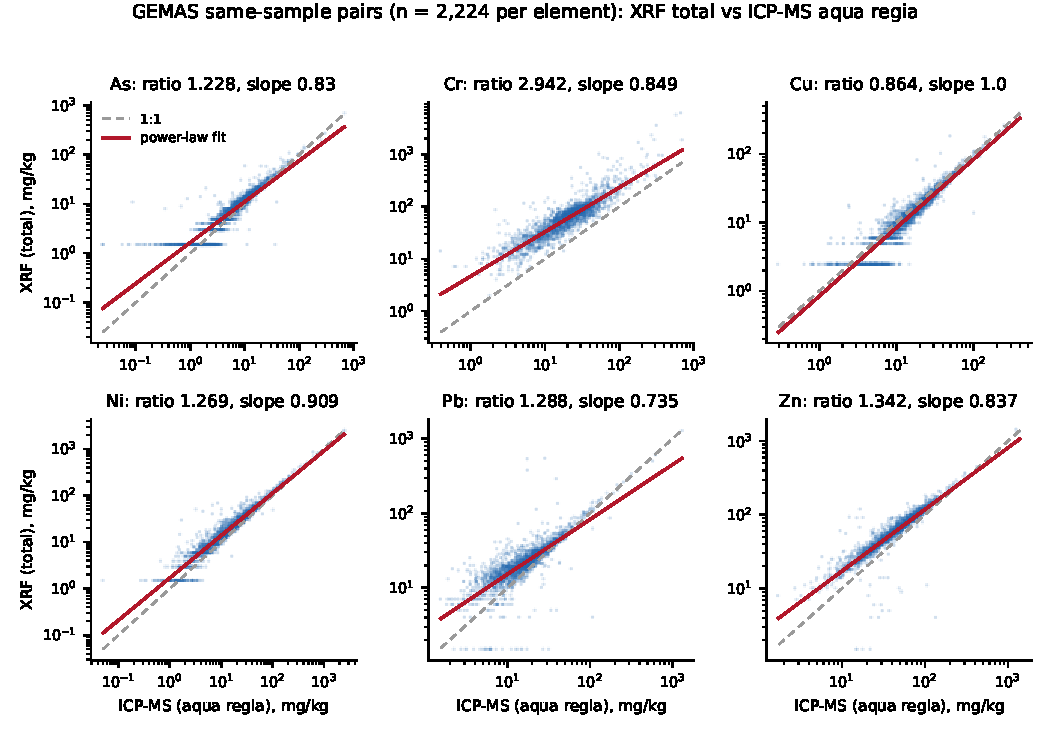
\includegraphics[width=\linewidth]{fig_p3_scatter.pdf}
\caption{GEMAS same-sample pairs ($n{=}2{,}224$ per element): XRF total
against ICP-MS aqua-regia concentration on log-log axes. Dashed grey line:
1:1; red line: fitted power law (Eq.~\ref{eq:powerlaw},
Table~\ref{tab:gemas}). Horizontal banding at low concentrations reflects
detection-limit quantization of the reported values, retained as-is (no
imputation). Points are rasterized at source resolution.}
\label{fig:scatter}
\end{figure}

\begin{figure}[!t]
\centering
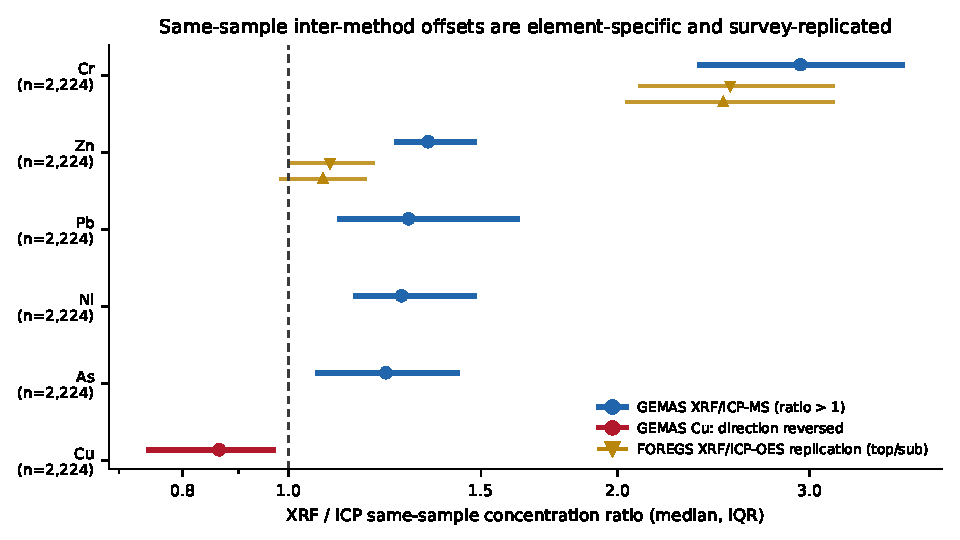
\includegraphics[width=0.86\linewidth]{fig_p3_forest.pdf}
\caption{Median same-sample ratios with IQR whiskers. Blue circles: GEMAS
XRF/ICP-MS; red circle: the direction-reversed Cu; gold triangles: FOREGS
XRF/ICP-OES replication on topsoil (down) and subsoil (up), shown for the
elements with same-sample double determinations (Cr, Zn;
Table~\ref{tab:foregs}). Log-scaled axis.}
\label{fig:forest}
\end{figure}

\begin{figure}[!t]
\centering

\includegraphics[width=\linewidth]{fig_p3_ba.pdf}
\caption{Bland--Altman (mean--difference) view of the same pairs:
$\log_2(\mathrm{XRF}/\mathrm{ICP\mbox{-}MS})$ against the geometric mean of
the two determinations. Solid red line: median offset; dashed red lines:
nonparametric 95\% limits of agreement (2.5th and 97.5th percentiles of the
per-sample log-ratios); gold curve: running median in twelve
concentration-quantile bins, whose tilt displays the concentration
dependence quantified by the slopes $b$ of Table~\ref{tab:gemas}. Dashed
grey line: zero offset.}
\label{fig:ba}
\end{figure}

Figure~\ref{fig:ba} recasts the same pairs in the Bland--Altman
(mean--difference) form standard in method-comparison studies
\cite{blandaltman1986}: per-sample $\log_2$ ratios against the geometric
mean of the two determinations, with the median offset and nonparametric
95\% limits of agreement (LOA). The LOA widths are the honest per-sample
uncertainty of any transfer: for Cr the central 95\% of same-sample ratios
span 1.49--6.86 --- even the 2.5th percentile sits half again above unity
--- while Zn is comparatively tight (1.06--2.22) and Cu straddles unity
(0.37--1.70). The tilted running medians anticipate the concentration
dependence quantified next.

\subsection{Offsets are concentration-dependent, and when that matters}
\label{sec:oos}
Slopes $b$ in Table~\ref{tab:gemas} range from 0.735 (Pb) to 1.000 (Cu):
for five of six elements the offset shrinks as concentration rises,
consistent with a roughly constant refractory or non-extractable component
that matters proportionally more in low-concentration samples. The
out-of-sample comparison (Table~\ref{tab:oos}) turns this observation into
a model-selection rule. For Pb --- the element farthest from $b{=}1$ ---
the power law cuts MdAPE from 18.2\% to 11.0\%, a 40\% error reduction; for
Zn the reduction is 17\%; for Cr, Ni and As the two models are within one
percentage point; and for Cu, whose slope is exactly 1.000, the constant
factor is marginally \emph{better} (13.5\% vs.\ 14.1\%), as expected when
the extra parameter fits noise. The practical rule shipped with the
transfer table is therefore: use the power law when $|b-1|$ exceeds its
standard error severalfold, otherwise the constant factor suffices.
Figure~\ref{fig:oos} shows the comparison directly: on the held-out Pb set
the constant-factor predictions fan away from the 1:1 line at both
concentration extremes --- exactly where a $b{=}0.735$ slope must defeat a
single multiplier --- while the power-law predictions stay centred; the
per-element bars restate Table~\ref{tab:oos} graphically.

\begin{figure}[!t]
\centering

\includegraphics[width=\linewidth]{fig_p3_oos.pdf}
\caption{Out-of-sample validation of the transfer models (seeded 80/20
split). Left: predicted versus observed XRF Pb on the held-out set under
the power-law (blue) and constant-factor (grey) models; dashed line: 1:1.
Right: held-out MdAPE per element for both models; labels give the relative
error reduction of the power law, negative for Cu where $b{=}1.000$ makes
the extra parameter pure noise.}
\label{fig:oos}
\end{figure}

\begin{table}[!t]
\centering
\caption{Out-of-sample validation (seeded 80/20 split): median absolute
percentage error (MdAPE) of predicting the held-out XRF value from the
ICP-MS value, for the power-law transfer model vs.\ a constant-factor
model. Gain is the relative MdAPE reduction of the power law.}
\label{tab:oos}
\small
\begin{tabular}{lccc}
\toprule
Element & Power law & Constant factor & Gain \\
\midrule
Pb & 0.110 & 0.182 & $+40\%$ \\
Zn & 0.062 & 0.075 & $+17\%$ \\
Cr & 0.203 & 0.211 & $+4\%$ \\
Ni & 0.116 & 0.117 & $+1\%$ \\
As & 0.173 & 0.173 & $0\%$ \\
Cu & 0.141 & 0.135 & $-4\%$ \\
\bottomrule
\end{tabular}
\end{table}

\subsection{Independent replication on FOREGS}
\label{sec:foregs}
FOREGS provides a genuinely independent check: different survey (1997--2001
vs.\ 2008--2009), different sample media (natural topsoil/subsoil vs.\
agricultural soil), and a different ICP instrument family (optical emission
rather than mass spectrometry). Where same-sample double determinations
exist (Cr, Zn), the offsets replicate in both magnitude and concentration
dependence (Table~\ref{tab:foregs}): Cr 2.54/2.50 (topsoil/subsoil) against
GEMAS 2.94, and Zn 1.09/1.08 against GEMAS 1.34. The Zn difference between
surveys (1.09 vs.\ 1.34) is itself informative: FOREGS ICP-OES follows a
stronger multi-acid protocol for some elements \cite{salminen2005}, so the
extractable fraction is survey-specific --- exactly why transfer models
must be estimated per survey pair rather than assumed universal, and why
the metadata standard of \S\ref{sec:standard} requires the digestion
protocol, not merely the instrument, to be recorded.

\begin{table}[!t]
\centering
\caption{FOREGS replication: XRF (total) vs.\ ICP-OES (partial digestion),
same-sample pairs. Layout as in Table~\ref{tab:gemas}.}
\label{tab:foregs}
\small
\begin{tabular}{llcccccc}
\toprule
Panel & El. & $n$ & Median ratio & 95\% CI & IQR & $b$ (SE) & $r^2$ \\
\midrule
Topsoil & Cr & 420 & 2.537 & 2.476--2.654 & 2.093--3.163 & 0.938 (0.023) & 0.805 \\
Subsoil & Cr & 417 & 2.500 & 2.429--2.600 & 2.036--3.160 & 0.891 (0.017) & 0.864 \\
Topsoil & Zn & 420 & 1.091 & 1.078--1.107 & 1.000--1.198 & 1.131 (0.018) & 0.906 \\
Subsoil & Zn & 417 & 1.075 & 1.062--1.100 & 0.982--1.179 & 1.261 (0.019) & 0.915 \\
\bottomrule
\end{tabular}
\end{table}

\section{Discussion}

\textbf{Consequences for data pooling.} If GEMAS aqua-regia and any
total-method Cr data were pooled uncorrected, the method split alone would
manufacture a factor-3 apparent difference --- larger than most genuine
regional contrasts in European soil Cr \cite{devos2006}. This is why the
harmonized database that hosts these records deliberately certifies zero
multi-source poolable cohorts until a transfer layer exists. The matrix in
Tables~\ref{tab:gemas}--\ref{tab:foregs} is that layer for its two largest
soil surveys: applied at the record level it converts ``cannot be
compared'' \cite{unep2025} into ``comparable within a quantified
uncertainty,'' with the OOS MdAPE of Table~\ref{tab:oos} serving as the
per-element uncertainty floor.

\textbf{When a constant factor is enough.} The slope criterion gives a
defensible, data-driven answer to a recurring practical question. Pb
($b{=}0.735$) and the other $b<1$ elements need the power law at
concentration extremes; Cu behaves as a clean proportional offset. Because
$b$ and its SE are part of the shipped table, a pipeline can make this
decision mechanically.

\textbf{Minimum method metadata.}
\label{sec:standard}
Every failure mode encountered in building the matrix traces to missing
metadata, not missing chemistry. We therefore propose that survey data
releases record, per determination: (1) instrument family (XRF, ICP-MS,
ICP-OES, \ldots); (2) digestion/extraction protocol with standard reference
(e.g.\ aqua regia per ISO 11466 \cite{iso11466}); (3) detection limit and
below-limit convention; (4) reference materials analysed in-batch; and (5)
a stable sample identifier enabling same-sample joins. GEMAS satisfies all
five --- which is precisely why this paper could be written from open data;
surveys missing item (5) can never contribute to a same-sample matrix,
whatever their analytical quality.

\textbf{Limitations.} The matrix covers two European surveys and six
elements; transfer functions are survey-pair-specific by construction and
must not be extrapolated to other digestion protocols (the FOREGS Zn case
demonstrates why). Detection-limit banding inflates ratio dispersion at low
concentrations for As and Cu; the OOS errors absorb this honestly but do
not remove it. Covariate modelling (pH, organic carbon, clay content) could
explain part of the residual spread and is queued as follow-up once those
covariates are harmonized into the snapshot.

\section{Conclusions}
Same-sample double determinations in open continental surveys make the
method-comparability problem quantifiable at zero laboratory cost. Across
2,224 GEMAS sample pairs per element, total-to-aqua-regia offsets range
from $-14\%$ (Cu) to $+194\%$ (Cr), are concentration-dependent for five of
six elements, and replicate independently in FOREGS. The resulting
transfer-model table --- medians, CIs, power-law parameters and
out-of-sample errors --- is published as a machine-readable layer, moving
harmonized open geochemistry from an honest ``zero poolable cohorts'' state
to conditional poolability with quantified uncertainty.

\section*{Data and code availability}
Input surveys: GEMAS \cite{reimann2014} and FOREGS
\cite{salminen2005,devos2006}, ingested with per-record licenses and
provenance hashes. The frozen snapshot identifier, analysis scripts
(\path{p345_full.py} and \path{p2345_addfigs.py}, seed 20260819),
result JSONs (\path{p345_full_results.json},
\path{p2345_addfigs_results.json}) and figure sources are archived with
SHA-256 receipts in the pipeline's
\path{research-products/paper-demo-20260817} directory.

\section*{Agent disclosure}
This draft, including analysis design, statistics, figures and text, was
produced end-to-end by an AI research agent operating the Global
Geochemical Atlas skill; the topic was proposed by the skill's
deterministic discovery-candidate generator (candidates dc-012--dc-016) and
has not yet completed human review. Screening-level framing is intentional
and load-bearing.

\begin{thebibliography}{9}
\bibitem{blandaltman1986}
Bland, J.M., Altman, D.G. (1986). Statistical methods for assessing
agreement between two methods of clinical measurement. \emph{The Lancet},
327, 307--310. doi:10.1016/S0140-6736(86)90837-8.

\bibitem{devos2006}
De Vos, W., Tarvainen, T. (chief eds.), et al. (2006). \emph{Geochemical
Atlas of Europe. Part 2: Interpretation of Geochemical Maps, Additional
Tables, Figures, Maps, and Related Publications}. Geological Survey of
Finland, Espoo.

\bibitem{eusml2025}
European Commission (2025). \emph{Soil Monitoring Law} (Directive on Soil
Monitoring and Resilience, in force 16 December 2025).
\url{https://environment.ec.europa.eu/topics/soil-health/soil-monitoring-law_en}.

\bibitem{iso11466}
International Organization for Standardization (1995). \emph{ISO 11466:
Soil quality --- Extraction of trace elements soluble in aqua regia}.
Geneva.

\bibitem{reimann2014}
Reimann, C., Birke, M., Demetriades, A., Filzmoser, P., O'Connor, P. (eds.)
(2014). \emph{Chemistry of Europe's Agricultural Soils} (GEMAS).
Geologisches Jahrbuch B102/B103, Schweizerbart, Stuttgart.

\bibitem{salminen2005}
Salminen, R. (chief ed.), et al. (2005). \emph{Geochemical Atlas of Europe.
Part 1: Background Information, Methodology and Maps}. Geological Survey of
Finland, Espoo.

\bibitem{unep2025}
UNEP Minamata Convention on Mercury, Open-Ended Scientific Group (2025).
\emph{Overview of monitoring, emission and release data}
(UNEP/MC/OESG.2/2/Rev.1) and OESG scientific report executive summary.
\url{https://minamataconvention.org}.
\end{thebibliography}

\end{document}
